\section{Cíl: první robot}

%\marginpar{Poznámka 1} % test poznámek - zdá se že fungují relativně dobře (PDF i HTML)
\fxnote*[author=JP]{Testovací poznámka k~prvnímu slovu ve větě - autor Jarek Páral (JP)}{Tento}
text je určen pro začátečníky a~mírně pokročilé v~oblasti stavby autonomních robotů -- převážně středoškoláky v~prvním ročníku, kteří se pokoušejí postavit svého prvního \hyperlink{autonomni}{autonomního}
%% co přesně dělá \link - reference do textu?
 %\link[ref:autonomni]{\color{blue}}{autonomního }\Black 
%\color{magenta} autonomního \color{black} 
robota, nejčastěji pro nějakou soutěž\footnote{Robotiáda v~Brně: 
\url{http://www.robotiada.cz/}, Robotický den v Praze \url{http://robotickyden.cz/} }. 
Protože byl sepsán na pracovišti Robotárna\footnote{\url{http://www.helceletka.cz/robotarna}} (pobočka DDM Helceletka Brno), jsou některé části určené především členům jeho kroužků. Ale většina textu je použitelná všeobecně.

Každý robot se musí 
\begin{itemize} 	% \itemsep = 0ex   
\item vyrobit (mechanická část -- konstrukce)
\item osadit elektronikou, motory a~pod.
\item naprogramovat 
\end{itemize}

Přitom můžou nastat zhruba dvě situace:

\begin{itemize} % \style O
\item  Nemám žádné znalosti a~zkušenosti $\rightarrow$ doporučený 
postup je začít ve školním kroužku nebo samostatně stavět a~programovat 
robota z~{\it Lego Mindstorms}\footnote{\url{https://www.lego.com/cs-cz/mindstorms}}.
Je to daleko nejjednodušší a~nejrychlejší cesta, omezení jste cenou stavebnice a~jejími možnostmi.
\item  Už jsem někdy něco naprogramoval nebo zapojil nebo postavil a~chci jít dál $\rightarrow$ potom je pro vás určen tento text.
Jednotlivé kapitoly se věnují různým oblastem, které je postupně potřeba zvládnout (nebo jimi pověřit jiného člena týmu) s~důrazem na začátečnické problémy.
\end{itemize}

\subsection{Týmy pro stavbu robotů}

Už bylo zmíněno, že stavba robotů zahrnuje tři propojené, 
ale relativně nezávislé okruhy: návrh a~výrobu mechanické konstrukce, 
návrh a~zapojení elektroniky a~programování.
Proto je dobré roboty stavět v~týmech, kde se jednotliví členové zaměřují na tyto oblasti a~navzájem se doplňují.
Navíc každý tým potřebuje řadu pomocných činností (nákup součástek, vyhledávání údajů na internetu a~pod.).
Je dobré mít proto v~každém týmu ještě pomocníka, který podporuje ostatní a~umožňuje jim soustředit se na jejich hlavní úkoly.

Úplně ideální potom je, když každou funkci v~týmu zastávají dva lidé, takže se mohou vzájemně zastupovat.
Tým by potom měl celkem osm členů -- dva mechaniky, dva elektroniky, dva programátory a~dva pomocníky.
To se ale v~praxi téměř nikdy nepodaří.
Často nastane právě opačný případ, kdy tým má pouze dva nebo tři členy, kteří se o~všechny činnosti musí nějak podělit.

V~každém případě ale platí, že je výhoda, pokud lidé v~týmu znají i~věci mimo jejich \uv{hlavní obor}, tj. když například programátor zná základy elekroniky.

\subsection{Postup návrhu robota}

\begin{enumerate} % \style n
\item  stanovit, co by měl robot splnit -- přibližně 
\item  sepsat, co by měl robot splnit -- podrobně (klidně i~více stran A4), z~toho vyplyne
\item  zjištění, jaké senzory a~pohony robot potřebuje a~kde budou na robotovi umístěné
\item  návrh první konstrukce robota včetně umístění senzorů a~pohonů
\item  zprovoznění toho všeho -- {\bf hlavní cíl tohoto textu }
\end{enumerate}

Začátečníci obvykle tuto posloupnost nedodrží a~pak staví mechaniku pro 3 a~více robotů, než zjistí, že je to dost práce navíc.
A~taky dost času navíc, který potom před soutěží může chybět. 

% na základě vlastních zkušeností s důkladnějším komentářem míst, kde jsem se zasekal (což bylo dost často :-) ).


\subsection{Co potřebujete na začátku}

{\bf Hardware: }

\begin{itemize} 
\item  notebook nebo počítač s~operačním systémem Windows 7 a~novějším nebo Linux (pro starší počítače např. aktuální distribuci Xubuntu, Lubuntu, Mint)
\item  desku s~čipem, např. DevKit ESP32\footnote{varianta: jinou vývojovou desku, např. Arduino Uno, Arduino nano, ...  }
\item  vývojovou desku ALKS\footnote{\url{https://github.com/RoboticsBrno/ArduinoLearningKitStarter} \newline {\color{red} NUTNÁ AKTUALIZACE} %todo NUTNÁ AKTUALIZACE desky na webu 
Hotová deska vás hlavně ze začátku zbavuje nutnosti vědět, co si můžete dovolit kam připojit a~hlavně nutnosti vůbec nějaké připojování čehokoliv řešit. }
\item výhledově cokoli dalšího, co chcete tím čipem řídit (serva, ultrazvuk, senzory a~motory všeho druhu ... )
\end{itemize}

\noindent {\bf Software: }
\begin{itemize} 
\item  {\it Visual Studio Code} -- viz kapitola \ref{vsc}
\item  {\it PlatformIO }-- viz kapitola \ref{platformio}
\end{itemize}
Veškerý zde popisovaný a~doporučovaný software je freeware.

\vspace*{1ex}

\noindent {\bf Znalosti:  }
\begin{itemize} 
\item  běžná práce se soubory ve vašem operačním systému (hledání, kopírování, mazání, ... )
\item  základy programování C++ (viz kapitola \ref{cpp}) a~příkazy C++ pro čipy (viz kapitola \ref{cppcipy})
\item  velmi se hodí schopnost porozumět textu psanému v~jednoduché angličtině)
\item  základy elektroniky -- viz kapitola \ref{elektronika}
\end{itemize}

\vspace*{1ex}

\noindent {\bf Taky se hodí vědět, že:  } 
\begin{itemize} 
\item veškeré \color{mygreen} zelené\color{black} \ a~\color{blue} modré \color{black} 
 \color{black} odkazy a~slova jsou proklikávací (s~výjimkou barevného zvýraznění 
syntaxe\footnote{syntaxe -- způsob zápisu daného jazyka, barevný zápis je mnohem přehlednější} ve zdrojových textech jazyka C++)
\item na konci textu je (klikací) obsah 
\item těsně před obsahem je (také klikací) rejstřík
\item v žádném textu o elektronice a robotice nemůže být všechno, pokud zde něco nenajdete, použijte např. Google
%\item tento text slouží pro \uv{začátečnický rozjezd}, pravděpodobně vám proto časem přestane stačit
\end{itemize}

\subsection{První projekt}
 

 
%\nonum \notoc 
\subsubsection*{Postup}

Pokud s~programováním čipů začínáme, čekají nás tyto úkoly:
\begin{enumerate}
\item  nainstalovat prostředí {\it Visual Studio Code}
\item  do VS Code nainstalovat tzv. {\it PlatformIO }
\item  založit nový projekt
\item  napsat zdrojový kód, přeložit a~dostat jej do čipu 
\end{enumerate}
Toto vše podrobněji probereme na dalších řádcích. 

\label{vsc} \subsubsection{Nainstalovat  Visual Studio Code} \label{vscode}

%% \index{neco} % pokud chci mít slovo v indexu a v textu, musím jej zopakovat - nenašel jsem v LaTeXu jinou možnost
{\it Visual Studio Code} \index{Visual~Studio~Code} (zkráceně VS Code) 
je něco jako textový editor, speciálně navržený pro programátory čehokoliv.
Instalujte podobně jako každý jiný program, stahujte zde: \url{https://code.visualstudio.com/}  


\subsubsection{Nainstalovat PlatformIO} \label{platformio}

\index{PlatformIO} PlatformIO je ten software, který umožní program v~C++ 
přeložit tak, aby ho čip pochopil a~taky ho do čipu umí nahrát. 
Instalace podle návodu zde: \url{http://docs.platformio.org/en/latest/ide/vscode.html\#installation}

\subsubsection{Založit nový projekt}

Program (ne)píšete jen do jednoho souboru, ale aby vše fungovalo, potřebujete povícero dalších souborů, které dohromady tvoří tzv. {\bf projekt}\index{projekt}.
Tyto soubory jsou mezi sebou hodně provázané a~navíc vázané na konkrétní místo uložení, 
takže vám po překopírování na jiný počítač pravděpodobně program nepůjde přeložit a~nebo 
nahrát do čipu. Řešení: uložit celý projekt na flešku. 
Na novém počítači založit nový projekt a~potřebné části zdrojového kódu kopírovat pomocí Ctrl+C, Ctrl+V. 

\begin{enumerate}
\item  Založte nový projekt z~ikonky \uv{domeček} -- viz \url{http://docs.platformio.org/en/latest/ide/vscode.html\#quick-start}.
\item  Do kolonky {\it Board} se musí vybrat správná deska.
Desek je přes 400 a~jsou rozdělené do sekcí řazených podle abecedy vyznačených šedivou barvou.
V~sekcích jsou potom jednotlivé desky řazené taky abecedně.
Pro čip ESP32 najdete sekci {\it Espressif32} a~v~ní položku {\it Espressif ESP32 Dev Module}.
Kolonka {\it Framework } se potom vyplní automaticky. 
\item  Zbývá vybrat adresář, do kterého bude projekt uložen.
Tento adresář si předem vytvořte, s~adresářem vytvářeným za pochodu má VS Code kdovíproč problém.
Odškrtněte zatržítko {\it Use defalut folder} a~zvolte vytvořený adresář.  
\end{enumerate}

Pro Linux Lubuntu: projekt musí být uložen na pevném disku, ne na flešce, jinak prostě nepojede, netuším proč.  

\subsubsection{Napsat zdrojový kód, přeložit a~dostat jej do čipu}

\begin{figure}[h]
	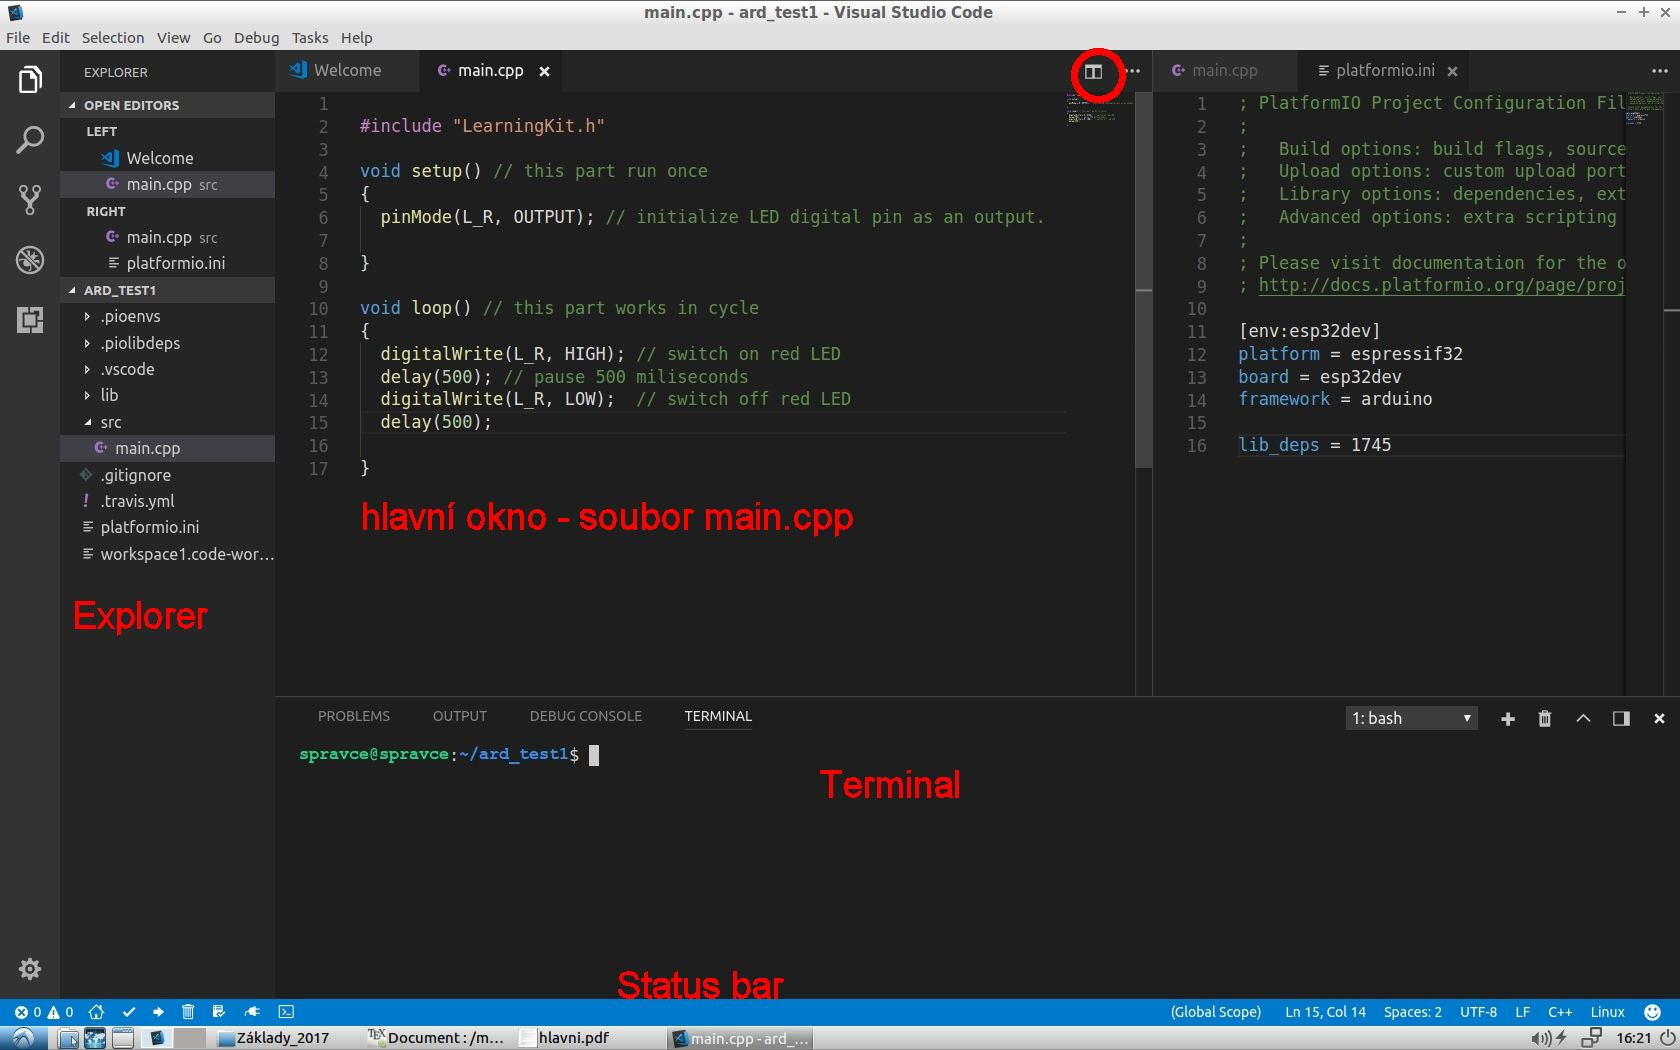
\includegraphics[width=\textwidth]{soubory/rozlozeni2.jpg}
	\caption{Rozložení oken v~programu {\it VS Code}} 
	\label{fig:vsc_rozlozeni}
\end{figure}	

\hypertarget{explorer}{}
Obrázek \ref{fig:vsc_rozlozeni} na straně~\pageref{fig:vsc_rozlozeni} ukazuje rozložení oken v~rámci projektu.
Hlavní okno  rozdělte na dvě části pro zobrazení dvou upravovaných souborů pomocí ikony v~kroužku.
Začínáme v~okně {\bf Explorer}, \index{Explorer}
 kde je umístěna adresářová struktura projektu\footnote{Pokud toto okno není vidět, zobrazíte ho v~menu {\it View} položka {\it Explorer} }.
Otevřete soubory {\it platformio.ini} a~v~adresáři {\it src} soubor {\it main.cpp}. 
 
Pro pohodlnou práci s~deskou ALKS byla \index{LearningKit} napsaná tzv. knihovna {\it LearningKit}. 
Aby fungovala, musí být do souboru {\it platformio.ini} dopsán řádek {\tt lib\_deps = 1745} (bez mezery na začátku řádku) a~do záhlaví souboru {\it main.cpp} doplňte
% {\tt include "LearningKit.h\"}.  
%% nahrazeno \verb| include "LearningKit.h"|
\verb| include "LearningKit.h"|
Dále dopište do souboru {\it main.cpp} kód, který bliká červenou LED.
Vše je vidět na obrázku \ref{fig:vsc_rozlozeni}.
Celý zdrojový kód tohoto prvního programu (obsah souboru {\it main.cpp}) je uveden v~kapitole \ref{cpppr1}.
 
Teď budou potřeba další dvě části VS Code: terminál \index{terminál} (okno vpravo dole) a~stavový řádek (Status~bar\index{Status~bar} -- proužek pod terminálem). 
Na stavovém řádku klikněte na ikonu šipky\footnote{totéž provede Ctrl+Alt+U} (pátá zprava) a~{\it PlatformIO} se pokusí váš program přeložit a~nahrát do čipu. 
Pokud chcete program pouze přeložit, klikněte na ikonu zatržítko\footnote{totéž provede Ctrl+Alt+B} hned vedle. 

Při prvním pokusu nahrát program do čipu na Linuxu může mít {\it PlatformIO} problém, že nenajde USB spojení na desku s~čipem a~vyžaduje ho doistalovat. 
Zpráva\footnote{\tt Warning! Please install `99-platformio-udev.rules`} se objeví se v~terminálu včetně nápovědy,\footnote{\url{https://raw.githubusercontent.com/platformio/platformio/develop/scripts/99-platformio-udev.rules}} jak to udělat.
Nápověda je ale tak podrobná, že to středně poučený linuxový laik s~pomocí internetu zvládne.
Při všech dalších překladech už to nebude problém.  

Další programy budou uvedeny v~kapitole \ref{cpppr}. 
